%%%%%%%%%%%%%%%%%%%%%%%%%%%%%%%%%%%%%%%%%%%%%%%%%%%%%%%%%%%%%%%%%%%%%%
% BAB TINJAUAN PUSTAKA
%=====================================================================
\renewcommand{\thechapter}{\Roman{chapter}}
\addtocontents{toc}{\vskip10pt}
\chapter{TINJAUAN PUSTAKA}
\renewcommand{\thechapter}{\arabic{chapter}}

%---------------------------------------------------------------------

%%%%%%%%%%%%%%%%%%%%%%%%%%%%%%%%%%%%%%%%%%%%%%%%%%%%%%%%%%%%%%
\section{Material 2D}
Material berdimensi dua (2D) merupakan sistem kristal di mana atom-atom tersusun dalam lapisan tunggal atau beberapa lapisan yang sangat tipis, dengan ikatan kovalen yang kuat secara \emph{dalam bidang (in-plane, IP)} dan interaksi van der Waals di antara lapisan.
Material ini telah menjadi fokus riset intensif sejak isolasi grafena pada tahun 2004 karena sifat mekanik, elektronik, dan termalnya yang unik \citep{Novoselov2004, Geim2007}.

\subsection{Deskripsi Material 2D}
Material 2D memiliki karakteristik yang membedakannya dari material tiga dimensi (3D).
Secara fisik, material 2D menunjukkan kestabilan yang tinggi meskipun hanya tersusun dari satu atau beberapa lapisan atom, di mana fenomena pengekangan kuantum (\textit{quantum confinement}, PK) menjadi sangat dominan.
Struktur ini memungkinkan pengamatan efek kuantum dalam skala makroskopik, sehingga mengubah properti elektronik seperti mobilitas pembawa muatan dan pita energi.
Sebagai contoh, grafena memiliki struktur sarang lebah (\textit{honeycomb}, SL) yang simetris yang menghasilkan pita konik (Dirac cones) pada titik K di Brillouin zone, sehingga elektron berperilaku seperti partikel dengan massa nol \citep{CastroNeto2009}.
Sejarah material 2D dimulai dari penemuan grafena dan berlanjut pada sintesis material seperti MoS\(_2\), WS\(_2\), dan hBN.
Metode isolasi mekanik, Deposisi Uap Kimia (CVD) serta eksfoliasi kimia telah banyak digunakan untuk memperoleh lapisan atom tunggal dengan kualitas kristal yang tinggi.
Studi awal berfokus pada grafena, namun perkembangan teknologi sintesis mendorong riset pada material lain dengan sifat semikonduktor atau isolator, seperti hBN yang memiliki pita energi lebar \citep{Geim2013}.
Material 2D umumnya ditandai dengan:
\begin{itemize}
    \item \textbf{Dimensi Terbatas:} Ketebalan material mendekati satu lapisan atom.
    \item \textbf{Anisotropi:} Sifat fisik seperti konduktivitas termal dan mekanik sangat bergantung pada arah dalam bidang (\emph{in-plane}, IP) dan lintas bidang (\emph{out-of-plane}, OP)).
    \item \textbf{Efek Kuantum:} Struktur elektron menunjukkan efek PK yang kuat, yang mengubah densitas keadaan elektron dan menghasilkan fenomena seperti efek Hall kuantum \citep{Das2015}.
\end{itemize}

\subsection{Sifat Struktural dan Mekanik}
Material 2D memiliki kekakuan IP yang sangat tinggi meskipun fleksibilitas lintas bidang (OP) relatif besar.
Struktur kristal dua dimensi yang sempurna menghasilkan simetri spasial yang tinggi dan kestabilan termodinamik yang mendasar.
Secara matematis, energi elastis \( U \) dapat dihitung melalui pendekatan teori elastisitas dua dimensi:
\begin{equation}
    U = \frac{1}{2} \int \left( C_{11}\epsilon_{xx}^2 + 2C_{12}\epsilon_{xx}\epsilon_{yy} + C_{22}\epsilon_{yy}^2 + 2C_{66}\epsilon_{xy}^2 \right) dA,
\end{equation}
di mana \( C_{ij} \) merupakan konstanta elastis dan \( \epsilon_{ij} \) adalah tensor regangan \citep{Lee2008}.
Persamaan ini mendasari perhitungan sifat mekanik seperti modulus Young dan modulus geser.
Dalam model elastisitas material 2D, analisis terhadap deformasi homogen dan non-homogen dapat dilakukan dengan pendekatan kontinuum.
Dengan menyusun persamaan keseimbangan mekanik dalam koordinat kartesian, diperoleh persamaan diferensial parsial yang menggambarkan distribusi tegangan:
\begin{align}
    \frac{\partial \sigma_{xx}}{\partial x} + \frac{\partial \sigma_{xy}}{\partial y} &= 0, \nonumber \\
    \frac{\partial \sigma_{yx}}{\partial x} + \frac{\partial \sigma_{yy}}{\partial y} &= 0.
\end{align}
Hubungan antara tegangan \( \sigma_{ij} \) dan regangan \( \epsilon_{ij} \) dihubungkan oleh hukum Hooke dalam bentuk tensor \citep{Timoshenko1970}.

\subsection{Sifat Elektronik dan Optik}
Secara elektronik, material 2D memiliki densitas keadaan yang berbeda dengan material 3D karena adanya pembatasan dimensi.
Model elektron bebas dua dimensi dapat dituliskan sebagai:
\begin{equation}
    E(\mathbf{k}) = \frac{\hbar^2 k^2}{2m^*},
\end{equation}
di mana \( \hbar \) adalah konstanta Planck tereduksi, \( k \) adalah bilangan gelombang, dan \( m^* \) adalah massa efektif elektron.
Untuk grafena, model relativistik menghasilkan hubungan linier:
\begin{equation}
    E(\mathbf{k}) = \hbar v_F |\mathbf{k}|,
\end{equation}
dengan \( v_F \) adalah kecepatan Fermi, yang menghasilkan sifat konduktivitas tinggi serta mobilitas pembawa muatan yang ekstrem \citep{Novoselov2004,CastroNeto2009}.
Teori pita energi untuk material 2D umumnya dikaji dengan menggunakan metode DFT atau model ikatan erat (\emph{tight-binding}, TB).
Model ikatan erat untuk grafena, misalnya, menghasilkan persamaan pita:
\begin{equation}
    E(\mathbf{k}) = \pm t \sqrt{1 + 4\cos\left(\frac{\sqrt{3}k_y a}{2}\right)\cos\left(\frac{k_x a}{2}\right) + 4\cos^2\left(\frac{k_x a}{2}\right)},
\end{equation}
di mana \( t \) adalah parameter \emph{hopping} dan \( a \) adalah parameter kisi.
Persamaan ini menunjukkan titik Dirac dan konik di sekitar titik K yang memberikan kontribusi pada sifat semimetalik grafena \citep{CastroNeto2009}.

\subsection{Sifat Termal dan Transportasi}
Secara termal, material 2D menunjukkan konduktivitas termal yang tinggi di bidang IP karena adanya fonon dengan laju penyebaran tinggi.
Konduktivitas termal \(\kappa\) dapat dihitung menggunakan persamaan Boltzmann:
\begin{equation}
    \kappa = \frac{1}{A} \sum_{\lambda} C_{\lambda} v_{\lambda}^2 \tau_{\lambda},
\end{equation}
di mana \( C_{\lambda} \) adalah kapasitas panas per mode, \( v_{\lambda} \) adalah kecepatan grup fonon, dan \( \tau_{\lambda} \) adalah waktu relaksasi \citep{Das2015}.
Model ini sangat relevan untuk mengkaji transportasi termal pada material 2D seperti grafena dan hBN.
Karena pembatasan dimensi, banyak fenomena kuantum yang tidak terlihat pada material 3D dapat diobservasi.
Misalnya, efek Hall kuantum dan osilasi Shubnikov-de Haas muncul pada material 2D pada medan magnet kuat, serta fenomena lokalitas Anderson pada sistem tak teratur.
Efek kuantum ini dijelaskan melalui persamaan Schrödinger yang dimodifikasi untuk sistem dua dimensi dan melalui pendekatan \emph{Green’s function} \citep{Ando2002}.

\subsection{Aplikasi dan Prospek Riset Material 2D}
Material 2D telah diaplikasikan dalam berbagai bidang, mulai dari elektronik, sensor, hingga fotonik.
Struktur atom tunggal memungkinkan miniaturisasi perangkat dengan performa tinggi. Sebagai contoh, grafena digunakan dalam transistor, sensor gas, dan material konduktif fleksibel, sedangkan hBN sering digunakan sebagai substrat atau isolator karena kestabilannya dan minimnya cacat yang signifikan \citep{Geim2013}.
Integrasi material 2D dengan teknologi nanoelektronik membuka peluang untuk membuat perangkat dengan efisiensi tinggi dan konsumsi daya rendah.
Studi terkini menunjukkan bahwa penggabungan grafena dengan hBN dapat menghasilkan heterostruktur yang memiliki mobilitas tinggi dan stabilitas termal yang baik \citep{Wang2017}.
Pendekatan teoretis dan simulasi komputasional (misalnya, DFT dan MD) memainkan peran penting dalam memahami sifat material 2D.
Model simulasi memberikan pandangan mendalam mengenai interaksi antar atom, dinamika elektron, dan respons terhadap medan eksternal.
Oleh karena itu, pendekatan multidisipliner antara eksperimen, teori, dan simulasi sangat diperlukan untuk pengembangan material 2D di masa depan \citep{Das2015}.

%%%%%%%%%%%%%%%%%%%%%%%%%%%%%%%%%%%%%%%%%%%%%%%%%%%%%%%%%%%%%%
\section{hBN}

Hexagonal boron nitride (hBN) merupakan salah satu material 2D yang sangat menarik karena kesamaan strukturalnya dengan grafena namun memiliki sifat isolator yang unik.
hBN memiliki struktur kristal \emph{hexagonal} yang stabil dan menunjukkan sifat fisik, elektronik, magnetik, dan termal yang khas.

\subsection{Struktur Kristal hBN}

\begin{figure}[ht]
    \centering
    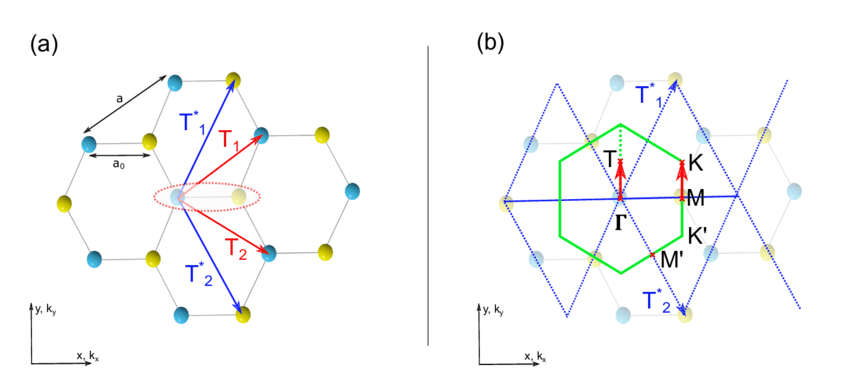
\includegraphics[width=0.8\textwidth]{gambar/hBN_structure_brillouinzone}
    \caption{Ruang resiprokal dan zona Brillouin pertama untuk h‑BN 2D.
(a) Bravais lattice lapisan tunggal BN: $\mathbf{T}_1$ dan $\mathbf{T}_2$ adalah vektor gelombang primitif, sedangkan $\mathbf{T}_1^*$ dan $\mathbf{T}_2^*$ adalah vektor gelombang resiprokal.
(b) Kisi resiprokal lapisan tunggal h‑BN yang diproyeksikan ke atas kristal.
Zona Brillouin pertama (diarsir hijau) untuk monolayer BN menunjukkan titik–titik simetri tinggi: $\Gamma$, K, M, K′, dan M′.
Pada kedua skema, bola kuning merepresentasikan atom Boron dan bola biru merepresentasikan atom Nitrogen.
\citep{elias2020}}
    \label{fig:reciprocal_bz_hbn}
\end{figure}

hBN tersusun dari lapisan atom boron (B) dan nitrogen (N) yang terikat secara kovalen dalam struktur  SL. Setiap atom boron terikat dengan tiga atom nitrogen dan sebaliknya, menghasilkan susunan yang hampir identik dengan grafena, dengan perbedaan jenis atom. Parameter kisi hBN dapat dinyatakan sebagai:
\begin{equation}
a = b \approx 2.50 \, \text{\AA}, \quad \gamma = 120^\circ.
\end{equation}

Persamaan ini mendasari simetri ruang dan menentukan bentuk Zona Brillouin yang juga berbentuk \emph{hexagonal}.

Struktur sarang lebah hBN, meskipun secara topologis identik dengan grafena, memiliki basis dua atom yang berbeda (satu B dan satu N) pada kisi Bravais segitiga. Vektor kisi primitif di ruang nyata dapat didefinisikan sebagai $\mathbf{a}_1 = a(1, 0)$ dan $\mathbf{a}_2 = a(1/2, \sqrt{3}/2)$. Dengan menggunakan hubungan definisi, vektor kisi resiprokal dapat diturunkan menjadi $\mathbf{b}_1 = \frac{2\pi}{a}(1, -1/\sqrt{3})$ dan $\mathbf{b}_2 = \frac{2\pi}{a}(0, 2/\sqrt{3})$. Vektor-vektor ini membentuk kisi resiprokal yang juga heksagonal, namun terotasi 30° relatif terhadap kisi langsung. Zona Brillouin pertama yang dibentuk dari konstruksi Wigner-Seitz pada kisi resiprokal ini adalah heksagon yang ditunjukkan pada Gambar \ref{fig:reciprocal_bz_hbn}.

Perbedaan paling fundamental antara hBN dan grafena, yang menjadi sumber sifat isolatornya, berasal dari pelanggaran simetri inversi. Dalam grafena, kedua atom karbon dalam basis identik, sehingga terdapat pusat simetri inversi di tengah-tengah ikatan C-C. Simetri ini melindungi degenerasi pita energi di titik K dan K' di sudut BZ, yang menghasilkan kerucut Dirac dan sifat semimetalik. Sebaliknya, dalam hBN, atom Boron dan Nitrogen secara kimiawi tidak ekuivalen. Tidak ada operasi simetri yang dapat mengubah atom B menjadi N sambil mempertahankan struktur kristal. Akibatnya, simetri inversi terlanggar.

Pelanggaran simetri ini memiliki konsekuensi langsung pada struktur elektronik. Potensial \emph{on-site} untuk elektron pada atom B berbeda secara signifikan dengan potensial pada atom N yang lebih elektronegatif ($V_B \neq V_N$). Perbedaan potensial ini bertindak sebagai perturbasi yang kuat yang "memecah" degenerasi pita yang ada pada grafena di titik K. Pemecahan ini membuka celah pita energi (\emph{band gap}) yang sangat besar, berkisar antara 5 hingga 6 eV, seperti yang telah dikonfirmasi oleh perhitungan DFT dan eksperimen. Celah pita ini bersifat langsung (\emph{direct gap}) di titik K, yang berarti minimum pita konduksi dan maksimum pita valensi terjadi pada vektor gelombang yang sama.

Sifat celah pita yang besar dan langsung ini secara langsung menjelaskan mengapa hBN adalah isolator listrik yang sangat baik dan transparan terhadap cahaya tampak. Hal ini menjadikannya substrat yang ideal untuk perangkat elektronik berbasis grafena, karena dapat meminimalkan hamburan muatan dan menjaga mobilitas elektron yang tinggi. Lebih jauh lagi, sifat optiknya yang unik di rentang ultraviolet dalam membuatnya menjadi kandidat material yang menjanjikan untuk aplikasi optoelektronik canggih, seperti dioda pemancar cahaya (LED) dan detektor di spektrum UV-dalam. Prediksi teoretis mengenai struktur pita ini, yang dihitung menggunakan metode seperti DFT, dapat diverifikasi secara langsung melalui teknik eksperimental seperti \emph{Angle-Resolved Photoemission Spectroscopy} (ARPES), yang mampu memetakan dispersi energi elektron sebagai fungsi dari momentumnya di dalam Zona Brillouin.

Struktur ini sangat stabil secara termodinamika dan menunjukkan anisotropi yang jelas antara arah IP dan OP. Secara matematis, fungsi gelombang atomik dalam hBN dapat dijelaskan dengan basis fungsi Bloch. Jika \(\psi_{\mathbf{k}}(\mathbf{r})\) merupakan fungsi Bloch, maka:
\begin{equation}
    \psi_{\mathbf{k}}(\mathbf{r}) = e^{i\mathbf{k}\cdot\mathbf{r}} u_{\mathbf{k}}(\mathbf{r}),
\end{equation}
di mana \(u_{\mathbf{k}}(\mathbf{r})\) adalah fungsi periodik sesuai dengan kisi kristal. Pendekatan ini digunakan dalam perhitungan pita energi dan densitas keadaan melalui metode DFT dan model \emph{tight-binding} \citep{CastroNeto2009}.
Simetri kristal hBN berpengaruh pada distribusi densitas muatan dan vibrasi fonon. Analisis simetri menggunakan grup titik \(D_{6h}\) memungkinkan identifikasi mode vibrasi Raman dan infra merah yang khas. Persamaan karakteristik mode fonon dapat diuraikan dari model dinamika kisi:
\begin{equation}
    \omega^2 = \frac{4K}{m}\sin^2\left(\frac{qa}{2}\right),
\end{equation}
dengan \(K\) sebagai konstanta gaya dan \(m\) adalah massa atom efektif. Model ini membantu menjelaskan perbedaan respon vibrasi antara hBN dan grafena, terutama dalam konteks aplikasi optoelektronik \citep{Wang2017}.

\subsection{Sifat Fisik, Elektronik, Magnetik, dan Termal hBN}
hBN memiliki sifat-sifat yang sangat berbeda dibandingkan dengan grafena.
Sifat elektroniknya yang berupa pita energi lebar membuat hBN berperan sebagai isolator ideal dalam heterostruktur.
Secara umum, gap energi hBN berkisar antara 5 hingga 6 eV, sehingga secara elektronik tidak menghantarkan muatan dalam kondisi normal \citep{Zhang2020}.
Model pita energi hBN dapat dihitung melalui metode DFT dengan menggunakan persamaan Kohn-Sham:
\begin{equation}
    \left(-\frac{\hbar^2}{2m}\nabla^2 + V_{ext}(\mathbf{r}) + V_H(\mathbf{r}) + V_{xc}(\mathbf{r})\right)\psi_i(\mathbf{r}) = \epsilon_i \psi_i(\mathbf{r}),
\end{equation}
di mana \(V_{ext}\) adalah potensial eksternal, \(V_H\) adalah potensial Hartree, dan \(V_{xc}\) merupakan fungsional pertukaran-korelasi.
Perhitungan ini menunjukkan bahwa sifat semikonduktor dengan gap besar mendasari peran hBN sebagai lapisan isolasi dalam perangkat heterostruktur \citep{Zhang2020}.
Secara mekanik, hBN memiliki kekakuan \emph{dalam bidang (IP)} yang tinggi namun menunjukkan koefisien ekspansi termal yang berbeda dibandingkan dengan grafena.
Persamaan elastisitas linear dalam hBN dapat diekspresikan sebagai:
\begin{equation}
    \sigma_{ij} = C_{ijkl}\epsilon_{kl},
\end{equation}
di mana \(C_{ijkl}\) merupakan tensor elastisitas dan \(\epsilon_{kl}\) adalah tensor regangan.
Sifat termal hBN yang tinggi secara konduktivitas IP mendukung aplikasinya sebagai pendingin pasif pada perangkat nanoelektronik \citep{Zhang2020}.
Meskipun hBN secara intrinsik tidak menunjukkan momen magnetik, keberadaan cacat titik atau doping dengan unsur logam dapat menginduksi sifat magnetik lokal.
Model magnetik untuk cacat dapat dijelaskan melalui Hamiltonian Heisenberg:
\begin{equation}
    \mathcal{H} = -\sum_{\langle i,j \rangle} J_{ij} \mathbf{S}_i \cdot \mathbf{S}_j,
\end{equation}
di mana \(J_{ij}\) adalah parameter interaksi pertukaran dan \(\mathbf{S}_i\) merupakan vektor spin di situs \(i\).
Studi pertama-prinsip telah menunjukkan bahwa cacat seperti vacancy atau substitusi dalam hBN dapat memicu keadaan magnetik, yang berpotensi untuk aplikasi spintronik \citep{Zhang2020}.

\subsection{Potensi Aplikasi hBN}
hBN telah menunjukkan potensi aplikasi yang luas, terutama dalam pengembangan heterostruktur 2D.
Kegunaan hBN sebagai substrat atau lapisan isolasi pada perangkat grafena telah menekan fluktuasi permukaan dan meningkatkan mobilitas elektron.
Selain itu, hBN juga dipertimbangkan untuk aplikasi dalam sensor, optoelektronik, dan penyimpanan energi \citep{Wang2017}.
Heterostruktur grafena/hBN menunjukkan peningkatan mobilitas pembawa muatan karena pengurangan hamburan permukaan.
Desain perangkat berbasis heterostruktur tersebut dapat dianalisis dengan menggunakan model transfer matriks dan pendekatan \emph{tight-binding} untuk menghitung pita terkuantisasi \citep{CastroNeto2009}.
Sifat optik hBN yang stabil pada rentang ultraviolet serta konduktivitas termal yang tinggi memungkinkan penerapannya dalam optoelektronik.
Penggunaan hBN sebagai lapisan pelindung atau lapisan aktif dalam LED dan laser nano telah diusulkan, dengan perhitungan band structure yang mendukung desain perangkat optik tersebut \citep{Zhang2020}.
Selain sebagai komponen aktif, hBN juga berperan sebagai dielektrik yang ideal dalam struktur MOSFET dan sebagai substrat untuk material 2D lainnya.
Keunggulan hBN terletak pada kestabilan kimia dan isolasi elektrik yang tinggi, yang memungkinkan integrasi dengan material semikonduktor lainnya tanpa mengganggu mobilitas pembawa muatan.
Hasil simulasi dan eksperimen menunjukkan minimnya cacat antarmuka pada struktur hBN \citep{Bhimanapati2016}.

%%%%%%%%%%%%%%%%%%%%%%%%%%%%%%%%%%%%%%%%%%%%%%%%%%%%%%%%%%%%%%
\section{Studi Terdahulu Terkait hBN}
Bagian ini memaparkan tinjauan literatur yang mendalam mengenai penelitian eksperimental dan komputasional terkait hBN.
Studi-studi terdahulu mencakup pendekatan sintetis, karakterisasi struktur, perhitungan elektronik, serta simulasi dinamika molekuler dan DFT untuk memahami cacat, cacat, dan modifikasi sifat material hBN.

\subsection{Tinjauan Eksperimental}

\begin{figure}[htbp]
  \centering
  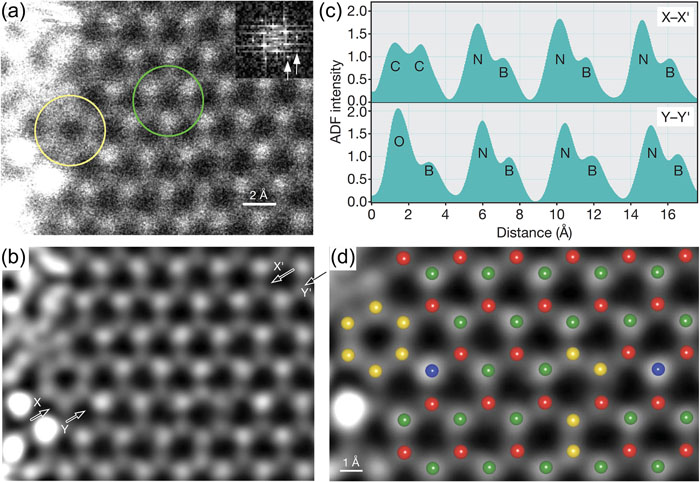
\includegraphics[width=0.9\textwidth]{gambar/hBN_stem.jpeg}
  \caption{Identifikasi substitusi atom pada monolayer h-BN menggunakan STEM yang dikoreksi aberasi. 
  (a) Citra ADF STEM monolayer h-BN yang direkam, dan 
  (b) citra ADF STEM hasil dekonvolusi. 
  (c) Profil garis dari intensitas ADF yang direkam sepanjang garis X--X′ dan Y--Y′ pada panel (b). 
  (d) Struktur atom h-BN hasil simulasi dengan atom pengotor substitusional (merah: B, kuning: C, hijau: N, dan biru: O) ditumpangkan pada citra ADF STEM hasil dekonvolusi. \citep{Zhang2020}}
  \label{fig:ADF_hBN_substitusi}
\end{figure}

Penelitian eksperimental mengenai hBN telah melibatkan teknik sintesis seperti eksfoliasi mekanik, CVD, dan epitaksi uap kimia.
Eksperimen karakterisasi menggunakan Raman spectroscopy, TEM, dan STM memberikan informasi mendetail mengenai struktur kristal, cacat titik, dan distribusi muatan elektron dalam hBN.
Sebagai contoh, studi oleh \citep{Bhimanapati2016} menunjukkan bahwa morfologi domain hBN pada substrat logam sangat bervariasi tergantung parameter sintesis, yang selanjutnya mempengaruhi sifat optik dan elektronik material.
Metode Raman spectroscopy telah digunakan untuk mengidentifikasi mode vibrasi khas pada hBN, memberikan informasi mengenai kekristalan dan adanya cacat.
Pengukuran intensitas puncak Raman serta pergeseran frekuensi mode \(E_{2g}\) menjadi indikator utama kualitas kristal \citep{Wang2017}.
Teknik TEM memungkinkan visualisasi struktur atomik hBN dengan resolusi sub-ångström.
Pengukuran konduktivitas termal dan respon magnetik hBN juga telah dilakukan secara eksperimental.
Teknik termal seperti time-domain thermoreflectance (TDTR) digunakan untuk mengukur konduktivitas termal IP, sedangkan studi magnetik dilakukan dengan magnetometri SQUID untuk mengidentifikasi pengaruh cacat terhadap sifat magnetik \citep{Zhang2020}.

\subsection{Tinjauan Teoritis dan Komputasional}
\begin{figure}[htbp]
  \centering
  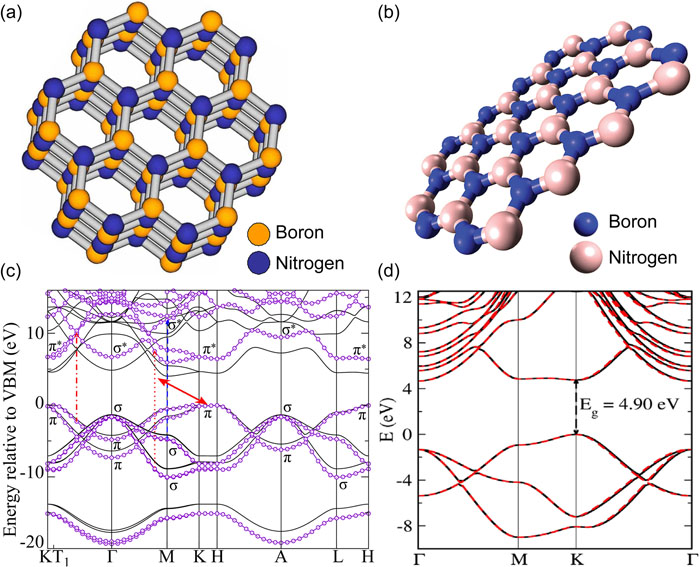
\includegraphics[width=0.9\textwidth]{gambar/referensi_band_plot.jpeg}
  \caption{Struktur atom dan pita energi h‑BN. 
    (a) Struktur atom bulk h‑BN. 
    (b) Struktur atom monolayer h‑BN. 
    (c) Struktur pita elektronik bulk h‑BN dihitung dengan LDA (garis hitam) dan GW (garis ungu). 
    (d) Struktur pita elektronik monolayer h‑BN dihitung melalui pendekatan DFT. \citep{Zhang2020}}
  \label{fig:hbn_atomic_band_structure}
\end{figure}

Pendekatan teoretis pada hBN melibatkan perhitungan DFT dan simulasi MD untuk memodelkan struktur elektronik, interaksi antar atom, dan dinamika cacat.
Studi oleh \citep{Lele2022} menggunakan ReaxFF-based molecular dynamics simulations untuk memprediksi morfologi domain hBN pada substrat nikel.
Metode ini melibatkan parameterisasi potensial reaktif yang memungkinkan simulasi reaksi kimia dan dinamika permukaan secara \emph{real-time}.
Dalam pendekatan DFT, persamaan Kohn-Sham digunakan untuk menghitung distribusi elektron dan energi total sistem hBN.
Metode ini diaplikasikan untuk mempelajari cacat titik, impuritas, dan efek doping.
Sebagai contoh, perhitungan pertama-prinsip menunjukkan bahwa substitusi atom atau kekosongan dapat menghasilkan keadaan elektronik baru yang mempengaruhi gap energi dan sifat magnetik lokal \citep{Zhang2020}.
Sebuah database densitas muatan yang \emph{representation-independent} telah dikembangkan untuk material kristalin, memfasilitasi perbandingan hasil perhitungan DFT dari berbagai metode dan potensial semu.
Pendekatan ini memverifikasi konsistensi data elektronik antara eksperimen dan simulasi, sehingga menjadi alat yang berguna dalam riset material hBN \citep{Shen2022}.

\subsection{Studi tentang Cacat dan Impuritas pada hBN}

\begin{figure}[htbp]
  \centering
  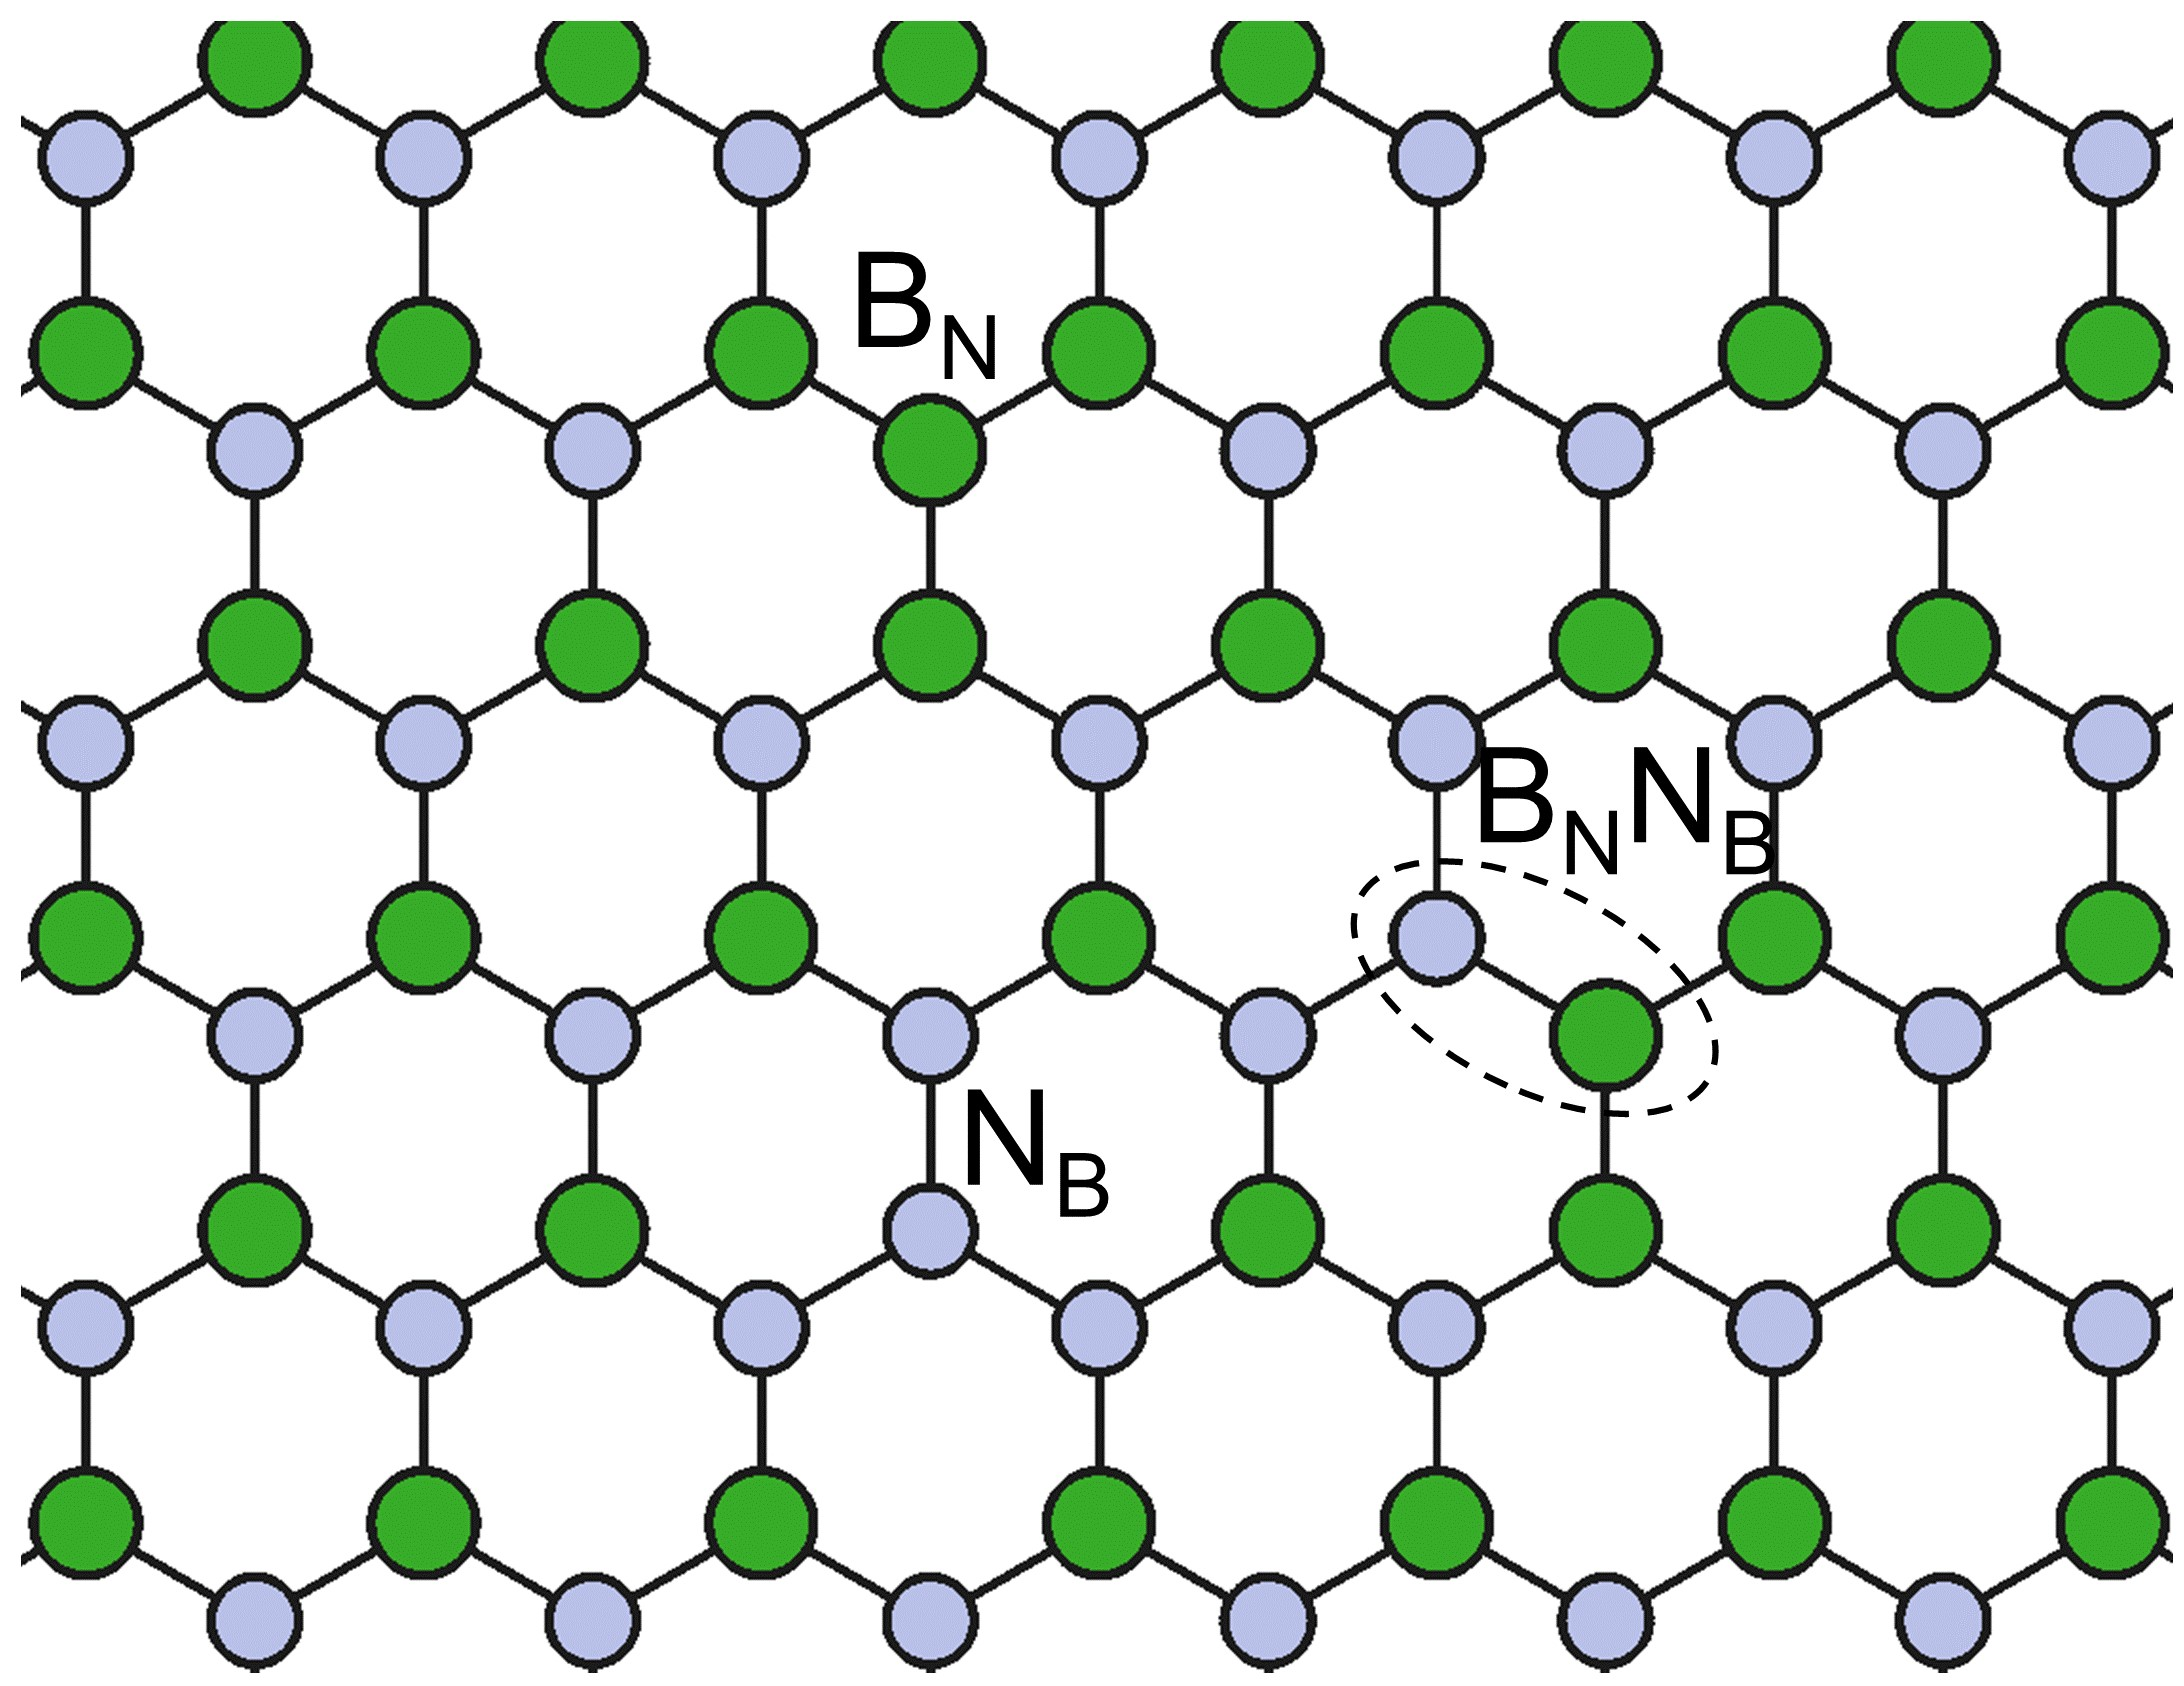
\includegraphics[width=0.8\textwidth]{gambar/antisite_hBN.jpg}
  \caption{Pandangan skematis cacat antisite asli $B_N$, $N_B$, dan $B_NN_B$. \citep{song2025}}
  \label{fig:schematic_antisite_defects}
\end{figure}

\begin{figure}[htbp]
  \centering
  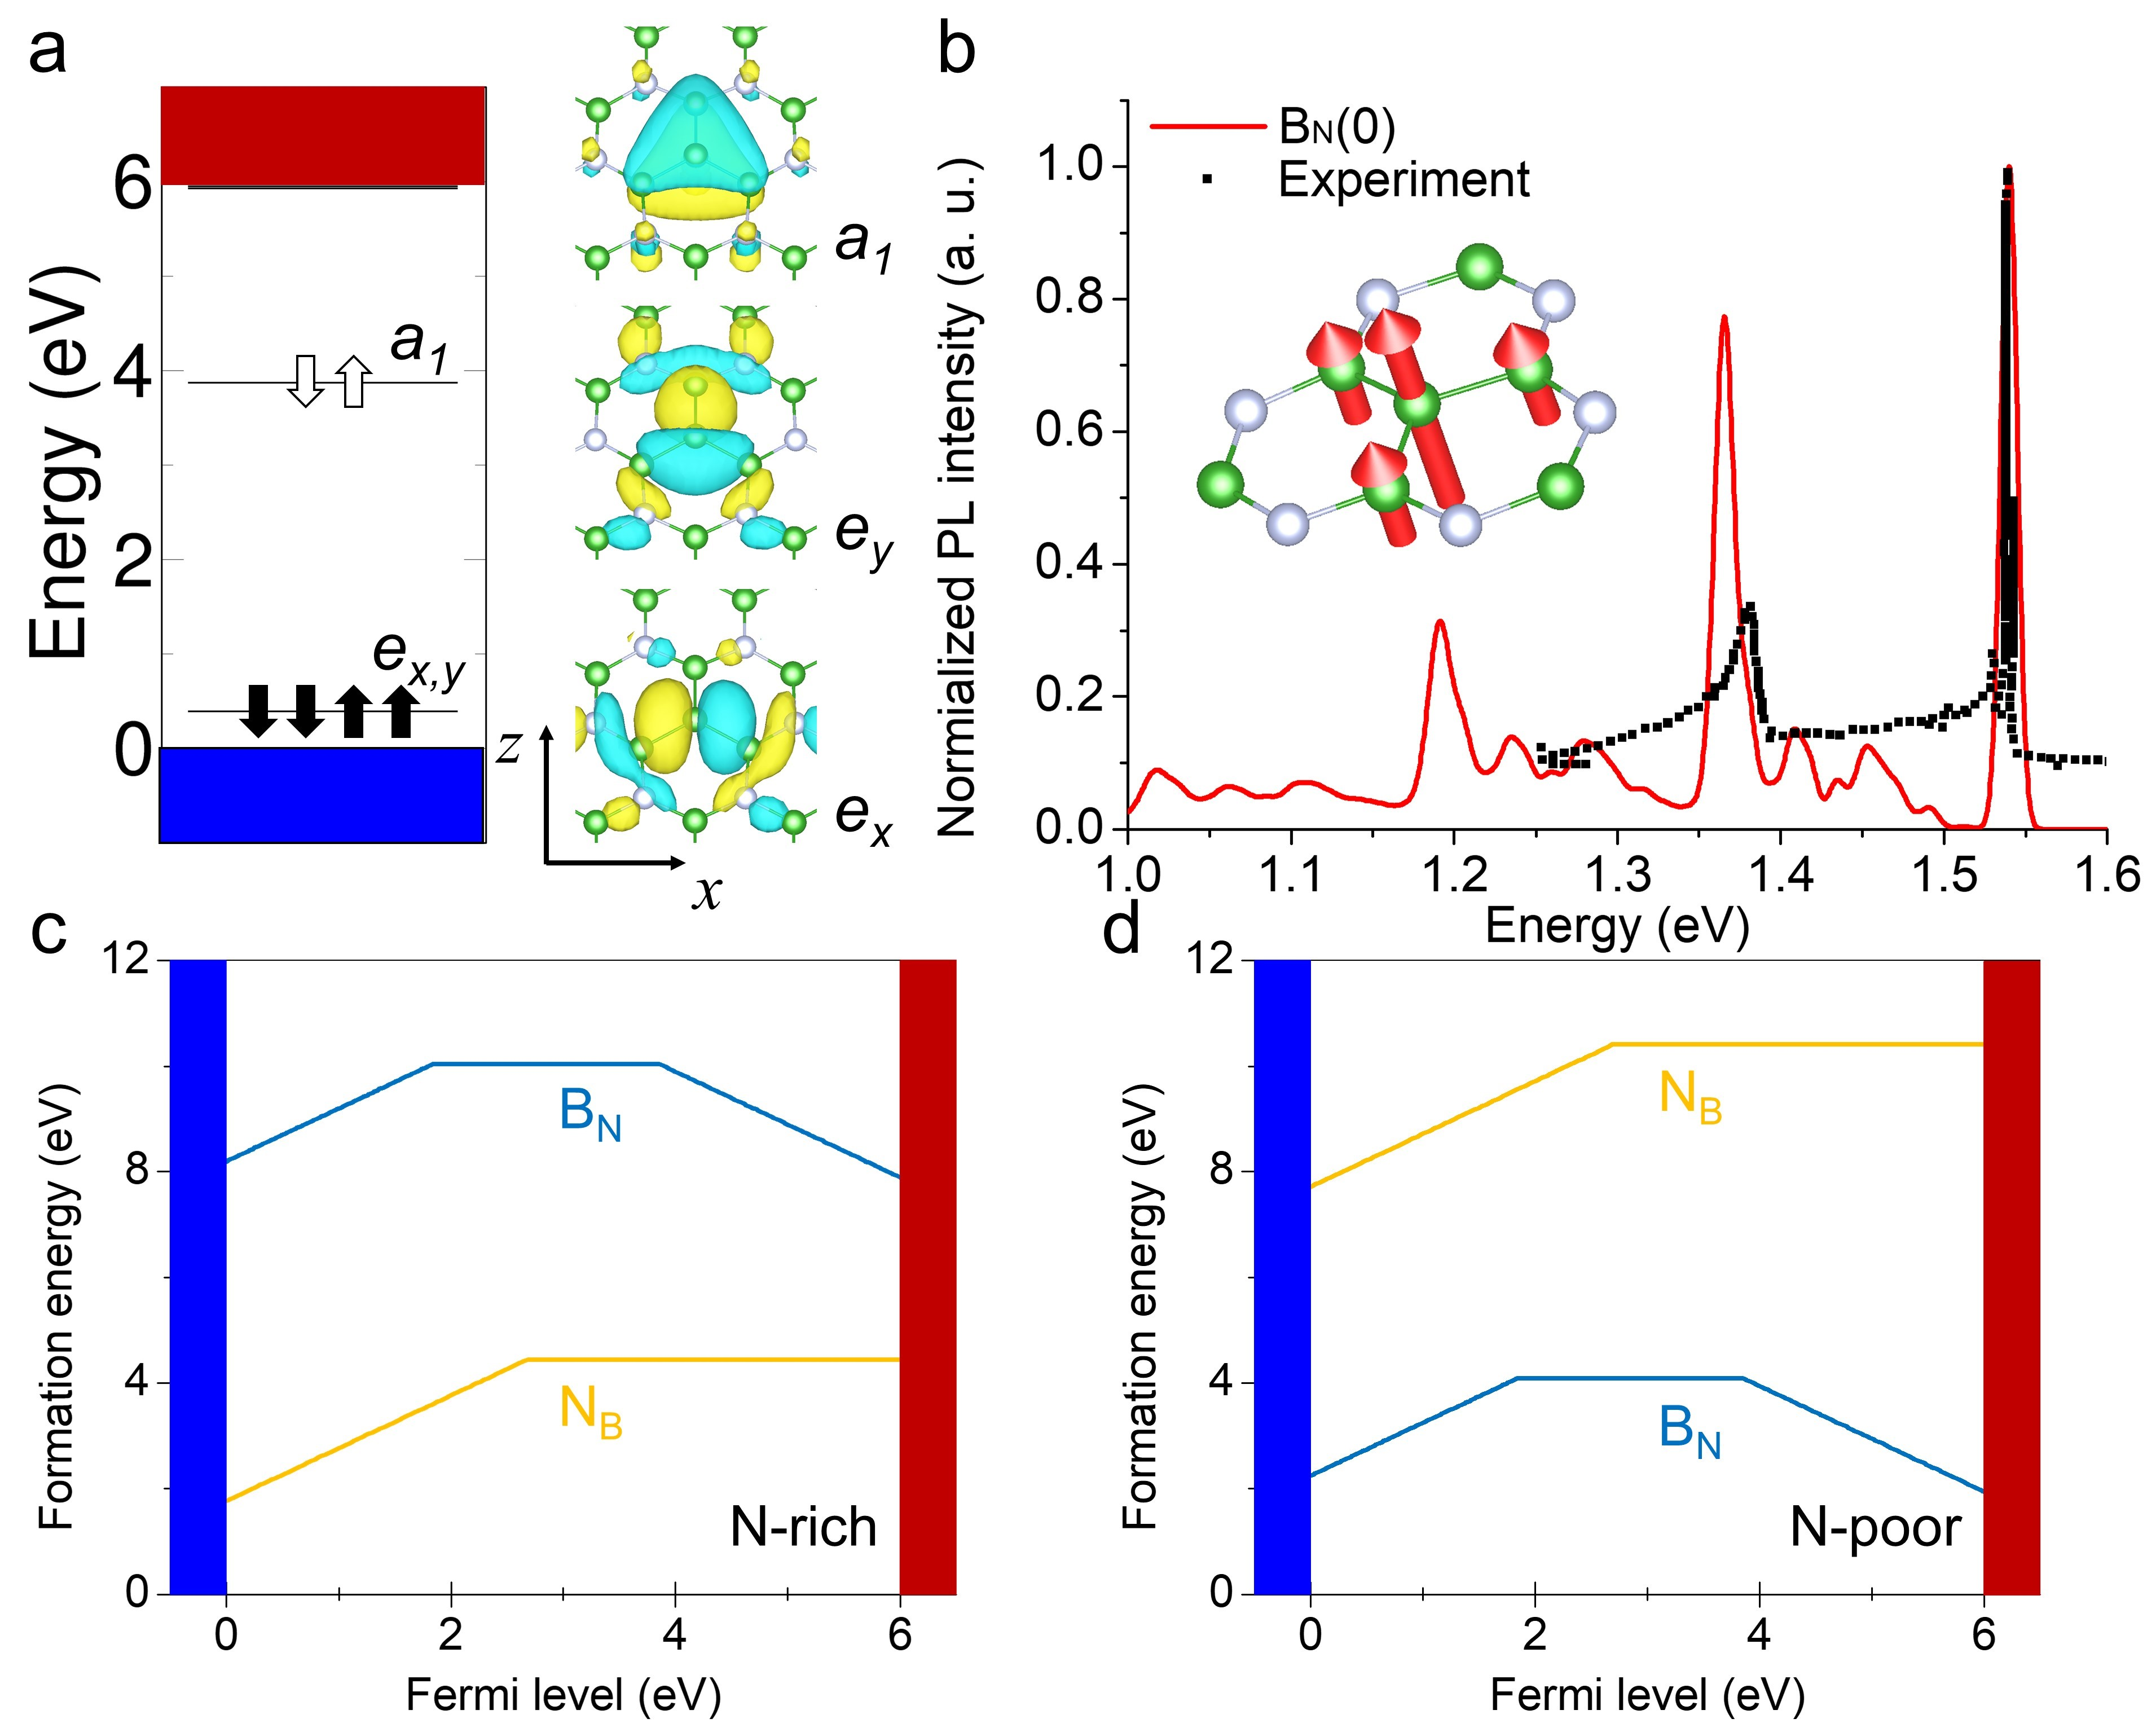
\includegraphics[width=0.9\textwidth]{gambar/elektronik_hBN_antisite.jpg}
  \caption{(a) Level energi keadaan dasar dari cacat BN(0) dengan simetri $\mathrm{C}_{3v}$ pada h‑BN. 
    (b) Spektrum PL eksperimental (Ref.\,31) dan simulasi. Inset menunjukkan mode getaran yang terkait dengan distorsi Jahn–Teller. 
    (c,d) Energi formasi $B_N$ dan $N_B$ pada kondisi kaya N dan miskin N. \citep{song2025}}
  \label{fig:BN0_JT_formation_energy}
\end{figure}
Penelitian mengenai cacat pada hBN sangat penting karena cacat dapat mengubah sifat elektronik dan magnetik material.
Berbagai studi telah menginvestigasi cacat titik seperti vacancy, interstisial, dan substitusi menggunakan simulasi DFT dan MD.
Hasil simulasi menunjukkan bahwa cacat dapat memicu keadaan lokal yang magnetik atau memodifikasi distribusi densitas elektron, sehingga berimplikasi pada aplikasi spintronik \citep{Zhang2020}.
Model cacat pada hBN dapat dijelaskan melalui pendekatan Hamiltonian modifikasi, dengan memasukkan tambahan potensial cacat \(V_d(\mathbf{r})\) ke dalam persamaan Kohn-Sham:
\begin{equation}
    \left[-\frac{\hbar^2}{2m}\nabla^2 + V_{ext}(\mathbf{r}) + V_H(\mathbf{r}) + V_{xc}(\mathbf{r}) + V_d(\mathbf{r})\right]\psi_i(\mathbf{r}) = \epsilon_i \psi_i(\mathbf{r}).
\end{equation}
Persamaan ini memungkinkan studi dampak cacat terhadap energi dan distribusi muatan elektron.
Perbandingan dengan data eksperimen mengkonfirmasi bahwa cacat dapat berperan sebagai pusat penangkapan pembawa muatan atau sumber \emph{scattering} \citep{Zhang2020}.

\subsection{Integrasi Studi Eksperimental dan Komputasional}
Pendekatan integratif antara eksperimen dan simulasi memberikan gambaran menyeluruh mengenai hBN.
Data eksperimental mengenai morfologi dan sifat fisik hBN telah dikonfirmasi melalui simulasi MD yang memanfaatkan potensial ReaxFF serta perhitungan DFT mendetail.
Studi komparatif ini tidak hanya meningkatkan pemahaman mekanisme pertumbuhan hBN, tetapi juga memandu pengembangan aplikasi praktis, misalnya dalam desain heterostruktur untuk perangkat nanoelektronik \citep{Lele2022}.
Simulasi dinamika molekuler menunjukkan bagaimana parameter suhu, tekanan, dan interaksi antar atom mempengaruhi morfologi domain hBN pada substrat logam.
Algoritma MD yang akan dibahas pada seksi berikutnya memberikan wawasan mengenai dinamika pertumbuhan dan penyebaran cacat pada skala atomik, sehingga menghasilkan model pertumbuhan yang realistis \citep{Lele2022}.
Selain studi di atas, berbagai publikasi lain mendukung hasil-hasil tersebut.
Misalnya, database densitas muatan elektronik yang \emph{representation-independent} memberikan basis yang kuat untuk memverifikasi perhitungan DFT pada berbagai material kristalin, termasuk hBN \citep{Shen2022}.

%%%%%%%%%%%%%%%%%%%%%%%%%%%%%%%%%%%%%%%%%%%%%%%%%%%%%%%%%%%%%%
\section{Dinamika Molekuler}
Dinamika Molekuler (MD) merupakan metode komputasional yang digunakan untuk mensimulasikan gerak dan interaksi antarpartikel (atom, molekul, atau sub-unit lainnya) secara temporal.
Metode ini berakar pada mekanika klasik, di mana evolusi sistem ditentukan melalui integrasi persamaan gerak Newton.
Pendekatan MD tidak hanya memberikan wawasan mengenai struktur statis tetapi juga memfasilitasi analisis sifat dinamis, transportasi, serta reaksi kimia pada berbagai skala, mulai dari sistem biomolekuler hingga material padat dan cair \citep{Allen1989,Frenkel2001}.
Penggunaan MD sebagai jembatan antara model mikroskopik dan observasi eksperimental telah memperkaya pemahaman kita mengenai fenomena termodinamika dan kinetika pada skala atomik.
Selain itu, MD menjadi alat penting dalam verifikasi teori dan perancangan material baru, terutama ketika eksperimen langsung sulit dilakukan.

\subsection{Persamaan Gerak dan Prinsip Dasar}
Dasar dari simulasi MD adalah persamaan gerak Newton yang dituliskan untuk partikel ke-\(i\) sebagai:
\begin{equation}
    m_i \frac{d^2 \mathbf{r}_i(t)}{dt^2} = \mathbf{F}_i(t),
\end{equation}
di mana \(m_i\) adalah massa, \(\mathbf{r}_i(t)\) adalah posisi vektor, dan \(\mathbf{F}_i(t)\) adalah gaya total yang bekerja pada partikel tersebut.
Gaya ini dihasilkan dari gradien negatif fungsi energi potensial total:
\begin{equation}
    \mathbf{F}_i = -\nabla_i U(\mathbf{r}_1, \mathbf{r}_2, \ldots, \mathbf{r}_N).
\end{equation}
Pendekatan ini mengasumsikan bahwa interaksi antar partikel dapat direpresentasikan oleh fungsi potensial \( U \), yang biasanya merupakan jumlah kontribusi dari interaksi dua sistem, tiga sistem, dan seterusnya.
Secara konsep, hal ini juga menyiratkan bahwa hukum kekekalan energi berlaku selama integrasi persamaan gerak, sehingga penggunaan algoritma integrasi yang konservatif, seperti algoritma Verlet, sangat esensial \citep{Allen1989}.

\subsection{Medan Gaya dan Potensial Interaksi}
Pemilihan model potensial sangat berpengaruh terhadap keakuratan simulasi MD.
Secara umum, potensial interaksi dapat dikategorikan ke dalam:
\begin{itemize}
    \item \textbf{Potensial Non-Bonded:} Seperti potensial Lennard-Jones, Morse, dan Coulomb, yang digunakan untuk menggambarkan gaya tarik-menarik dan tolakan antar partikel yang tidak terikat secara kimia.
    \item \textbf{Potensial Bonded:} Termasuk energi ikatan, sudut, dan torsi yang mendeskripsikan interaksi antar atom dalam satu molekul.
\end{itemize}
Untuk sistem yang memerlukan penanganan reaksi kimia atau perubahan ikatan, pendekatan potensial reaktif seperti ReaxFF telah banyak diaplikasikan.
ReaxFF mampu secara dinamis memodifikasi urutan ikatan dan parameter interaksi sesuai dengan lingkungan lokal atom, sehingga memungkinkan simulasi reaksi kimia yang kompleks \citep{Lele2022}.
Secara matematis, energi total dalam model ReaxFF dapat dituliskan sebagai:
\begin{equation}
    U_{\text{total}} = U_{\text{bond}} + U_{\text{over}} + U_{\text{under}} + U_{\text{angle}} + U_{\text{torsion}} + U_{\text{non-bond}},
\end{equation}
di mana:
\begin{itemize}
    \item \( U_{\text{bond}} \) merepresentasikan energi ikatan yang bergantung pada jarak antar atom.
    \item \( U_{\text{over}} \) dan \( U_{\text{under}} \) adalah koreksi untuk kondisi over- dan under-koordinasi.
    \item \( U_{\text{angle}} \) dan \( U_{\text{torsion}} \) menangkap kontribusi energi dari sudut ikatan dan rotasi di sekitar ikatan.
    \item \( U_{\text{non-bond}} \) meliputi interaksi non-ikatan seperti van der Waals dan gaya Coulomb.
\end{itemize}
Model ini memungkinkan penyesuaian parameter secara lokal dan telah terbukti efektif untuk mensimulasikan sistem material reaktif seperti hBN, di mana pembentukan dan pemutusan ikatan harus ditangani secara eksplisit \citep{Lele2022}.

\subsection{Ensemble dalam Simulasi MD}

\begin{figure}[htbp]
    \centering
    % Gambar 1
    \begin{subfigure}[b]{0.45\textwidth}
        \centering
        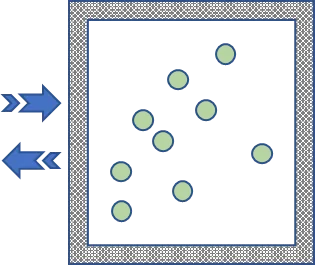
\includegraphics[width=\textwidth]{gambar/NVE.png}
        \caption{Ensemble NVE \\ (Energi total tetap)}
        \label{fig:nve}
    \end{subfigure}
    
    \vspace{1em}  % spasi vertikal antar gambar
    
    % Gambar 2
    \begin{subfigure}[b]{0.45\textwidth}
        \centering
        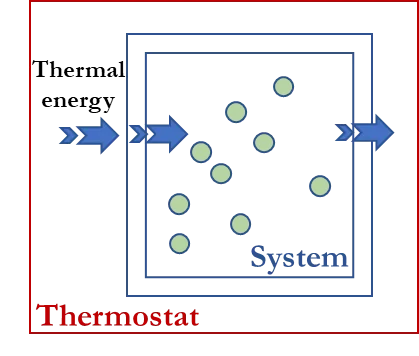
\includegraphics[width=\textwidth]{gambar/NVT.png}
        \caption{Ensemble NVT \\ (Suhu tetap)}
        \label{fig:nvt}
    \end{subfigure}
    
    \vspace{1em}
    
    % Gambar 3
    \begin{subfigure}[b]{0.75\textwidth}
        \centering
        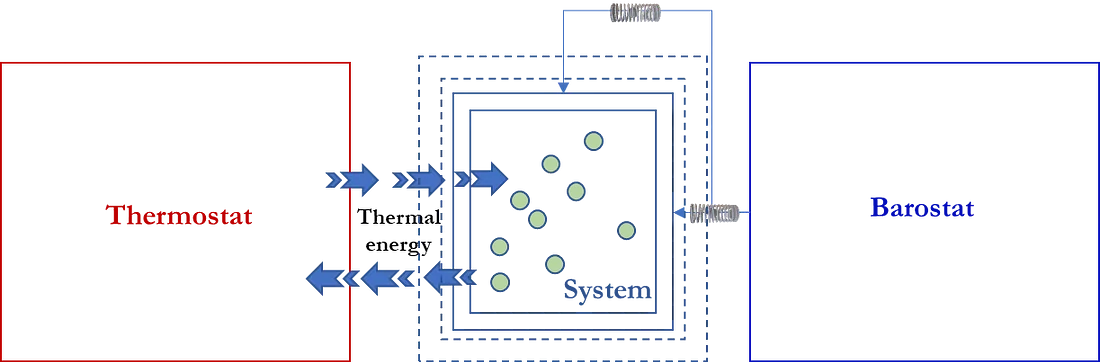
\includegraphics[width=\textwidth]{gambar/NPT.png}
        \caption{Ensemble NPT \\ (Tekanan tetap)}
        \label{fig:npt}
    \end{subfigure}

    \caption{Perbandingan visual tiga jenis ensemble dalam dinamika molekular: NVE, NVT, dan NPT.}
    \label{fig:ensemble_comparison}
\end{figure}

Agar hasil simulasi MD dapat merepresentasikan kondisi nyata, pemilihan ensemble (kumpulan kondisi termodinamika) sangat penting.
Beberapa ensemble yang umum digunakan antara lain:
\begin{itemize}
    \item \textbf{NVE (Microcanonical):} Energi, volume, dan jumlah partikel konstan.
    \item \textbf{NVT (Canonical):} Suhu konstan dengan penggunaan thermostat.
    \item \textbf{NPT (Isobaric-Isothermal):} Suhu dan tekanan konstan, yang penting dalam studi respons material terhadap perubahan eksternal.
\end{itemize}
Pemilihan ensemble menentukan distribusi probabilitas pada ruang fase. Sebagai contoh, untuk ensemble NVT, fungsi distribusi diberikan oleh:
\begin{equation}
    P(\mathbf{r}^N, \mathbf{p}^N) = \frac{1}{Z_{NVT}} \exp\left[-\beta H(\mathbf{r}^N, \mathbf{p}^N)\right],
\end{equation}
dengan \(\beta = 1/(k_B T)\) dan \(H\) merupakan Hamiltonian total sistem.
Distribusi ini menjamin bahwa rata-rata nilai termodinamika yang dihitung sesuai dengan prediksi teori statistik \citep{Kardar2007}.

\subsection{Algoritma Verlet dan Metode Integrasi Waktu}
Integrasi numerik persamaan gerak adalah aspek krusial dalam MD.
Algoritma Verlet, khususnya versi \emph{velocity Verlet}, banyak digunakan karena kestabilannya dan konservasi energi yang baik.
Persamaan dasar algoritma ini dituliskan sebagai:
\begin{equation}
    \mathbf{r}(t+\Delta t) = 2\mathbf{r}(t) - \mathbf{r}(t-\Delta t) + \frac{\mathbf{F}(t)}{m}\Delta t^2,
\end{equation}
dan versi \emph{velocity Verlet} yang juga menghitung kecepatan secara eksplisit:
\begin{align}
    \mathbf{v}(t+\Delta t) &= \mathbf{v}(t) + \frac{\mathbf{F}(t) + \mathbf{F}(t+\Delta t)}{2m}\Delta t, \\
    \mathbf{r}(t+\Delta t) &= \mathbf{r}(t) + \mathbf{v}(t)\Delta t + \frac{\mathbf{F}(t)}{2m}\Delta t^2.
\end{align}
Algoritma ini didasarkan pada pemisahan operator Liouville yang menjaga sifat-simetri waktu (\emph{time-reversibility}) dan simplektisitas, yang secara matematis memastikan bahwa volume ruang fase tetap terkonservasi.
Meskipun solusi numerik hanya mendekati lintasan eksak, algoritma Verlet secara efektif mempertahankan "Hamiltonian bayangan" yang konstan, sehingga tidak terjadi drift energi selama simulasi \citep{Allen1989}.

\subsection{Pengaturan Temperatur: Thermostat dan Barostat}
Pengaturan temperatur dalam simulasi MD dilakukan melalui penerapan thermostat, yang membantu menjaga sistem tetap berada dalam ensemble yang diinginkan.
Dua metode umum antara lain:
\begin{itemize}
    \item \textbf{Berendsen Thermostat:} Mengatur temperatur dengan menskalakan kecepatan partikel secara periodik, meskipun metode ini tidak menghasilkan distribusi canonical yang tepat.
    \item \textbf{Nose-Hoover Thermostat:} Memperkenalkan variabel tambahan (\(\xi\)) yang mengontrol fluktuasi energi sehingga menghasilkan distribusi canonical yang benar.
Persamaan geraknya adalah:
    \begin{equation}
        m_i \frac{d^2 \mathbf{r}_i}{dt^2} = \mathbf{F}_i - m_i \xi \frac{d\mathbf{r}_i}{dt},
    \end{equation}
    dengan dinamika \(\xi\) yang diatur melalui persamaan diferensial terkait energi kinetik \citep{Allen1989}.
\end{itemize}
Selain thermostat, penggunaan barostat juga penting untuk mensimulasikan sistem pada tekanan tetap (NPT), terutama dalam studi fase dan respon mekanis material.
Implementasi barostat biasanya melibatkan modifikasi pada volume sistem dan parameter interaksi, sehingga menjaga kestabilan tekanan selama simulasi.

\subsection{Implementasi Simulasi dengan LAMMPS}
LAMMPS (\emph{Large-scale Atomic/Molecular Massively Parallel Simulator}) merupakan salah satu paket perangkat lunak MD yang paling populer.
LAMMPS mendukung berbagai model potensial, termasuk potensial reaktif seperti ReaxFF, serta algoritma integrasi seperti Verlet dan Nose-Hoover.
Keunggulan LAMMPS antara lain:
\begin{itemize}
    \item Kemampuan untuk mensimulasikan sistem dengan jumlah partikel yang sangat besar.
    \item Fleksibilitas dalam mengatur kondisi batas, ensemble, dan parameter potensial.
    \item Dukungan untuk komputasi paralel yang efisien.
\end{itemize}
Dalam praktiknya, file input di LAMMPS harus mencakup definisi jenis interaksi (melalui potential file), parameter awal (koordinat, kecepatan, massa), serta pengaturan integrator dan thermostat/barostat.
Konfigurasi ini memungkinkan simulasi yang akurat dan efisien dalam mempelajari fenomena dinamis serta struktur material pada skala atomik \citep{Plimpton1995}.

\subsection{Pendekatan Lanjutan dan Implementasi Praktis MD}
Seiring dengan perkembangan metode simulasi, berbagai teknik lanjutan telah diintegrasikan ke dalam MD untuk menangani sistem yang lebih kompleks dan meningkatkan efisiensi perhitungan.
Beberapa pengembangan tersebut meliputi:
\begin{itemize}
    \item \textbf{Algoritma Multi-Timestep:} Untuk sistem dengan skala waktu yang berbeda, misalnya interaksi cepat berubah dan lambat berubah, algoritma multi-timestep memungkinkan penggunaan langkah waktu yang berbeda.
Metode ini memanfaatkan pemisahan gaya menjadi komponen cepat dan lambat, sehingga gaya cepat dihitung pada interval pendek, sedangkan gaya lambat dihitung lebih jarang \citep{Frenkel2001}.
    \item \textbf{Penanganan Kekangan (Constraints):} Dalam simulasi yang melibatkan ikatan dengan frekuensi tinggi, metode seperti SHAKE dan RATTLE digunakan untuk menjaga kekekangan pada panjang ikatan secara eksak, sehingga memungkinkan penggunaan langkah waktu yang lebih besar tanpa mengorbankan kestabilan numerik \citep{Frenkel2001}.
    \item \textbf{Pembagian Operator Liouville:} Pendekatan formal dengan memisahkan operator Liouville ke dalam komponen kinetik dan potensial memberikan dasar teoretis bagi algoritma integrasi seperti velocity Verlet.
Teknik ini tidak hanya memastikan konservasi energi (melalui Hamiltonian bayangan) tetapi juga sifat reversibilitas waktu dan simplektisitas \citep{Frenkel2001}.
    \item \textbf{Rotasi Molekul Kaku:} Untuk sistem dengan molekul non-sferis, perhitungan torsi dan rotasi molekul kaku sangat penting.
Pendekatan ini mengubah interaksi site-site menjadi gaya dan torsi pada pusat massa, sehingga mendukung simulasi dinamika rotasi \citep{Frenkel2001}.
\end{itemize}
Selain aspek algoritmis, penerapan praktis MD juga mencakup pembuatan sistem simulasi secara komprehensif.
Dalam studi modern, prosedur simulasi melibatkan:
\begin{itemize}
    \item Penentuan geometri awal dan pengaturan \emph{simulation box} dengan kondisi batas periodik, yang esensial untuk meminimalkan efek tepi.
    \item Penetapan kondisi awal, termasuk distribusi kecepatan berdasarkan distribusi Maxwell-Boltzmann, untuk memastikan replikasi kondisi termodinamika yang realistis.
    \item Penggunaan \emph{neighbour lists} untuk mengoptimalkan perhitungan gaya, terutama pada sistem dengan jumlah partikel yang besar.
\end{itemize}
Pendekatan praktis ini diilustrasikan dalam berbagai studi kasus, di mana MD tidak hanya digunakan untuk verifikasi teori tetapi juga untuk prediksi fenomena struktural dan dinamis pada sistem biologis, material padat, dan cair.
Teknik-teknik ini telah terbukti efektif dalam berbagai aplikasi, mulai dari simulasi protein hingga studi material dua dimensi, sebagaimana ditunjukkan dalam presentasi dan literatur terbaru \citep{Rapaport2004}.

%%%%%%%%%%%%%%%%%%%%%%%%%%%%%%%%%%%%%%%%%%%%%%%%%%%%%%%%%%%%%%
\section{ (DFT)}
 Teori Fungsional Kerapatan (\emph{Density Functional Theory}, DFT) merupakan salah satu metode komputasi kuantum yang paling banyak digunakan dalam studi struktur elektronik material.
Metode ini berfokus pada penggunaan densitas elektron \(\rho(\mathbf{r})\) sebagai variabel fundamental, bukan fungsi gelombang banyak partikel yang bergantung pada koordinat individual setiap elektron.
Dengan demikian, DFT menawarkan cara yang lebih efisien dalam menangani sistem dengan jumlah partikel yang besar, sekaligus memberikan akurasi yang memadai untuk banyak aplikasi dalam fisika material dan kimia komputasi \citep{Kohn1965, Martin2004}.
Pendekatan DFT telah merevolusi studi material karena mengurangi kompleksitas masalah banyak partikel melalui penggunaan prinsip-prinsip teorema Hohenberg-Kohn dan persamaan Kohn-Sham.
Meski demikian, keberhasilan DFT sangat bergantung pada pemilihan fungsional pertukaran-korelasi (\emph{exchange-correlation functional}) yang tepat.
Oleh karena itu, pemahaman mendalam terhadap dasar-dasar teoritis dan persamaan-persaamaan yang digunakan sangat penting bagi para peneliti.

\subsection{Persamaan Schrödinger}
Dasar perhitungan dalam mekanika kuantum untuk sistem banyak partikel adalah persamaan Schrödinger tak-relativistik:
\begin{equation}
    \hat{H}\Psi(\mathbf{r}_1,\mathbf{r}_2,\ldots,\mathbf{r}_N) = E\Psi(\mathbf{r}_1,\mathbf{r}_2,\ldots,\mathbf{r}_N),
\end{equation}
di mana \(\Psi\) merupakan fungsi gelombang yang mengandung informasi lengkap tentang keadaan sistem.
Fungsi gelombang ini bergantung pada koordinat semua elektron dalam sistem, sehingga ruang konfigurasi yang harus dipertimbangkan menjadi sangat besar seiring dengan bertambahnya jumlah partikel.
Hamiltonian \(\hat{H}\) untuk sistem elektron dalam medan potensial eksternal diberikan oleh
\begin{equation}
    \hat{H} = -\sum_{i=1}^{N}\frac{\hbar^2}{2m}\nabla_i^2 + \sum_{i<j} \frac{e^2}{4\pi\varepsilon_0|\mathbf{r}_i-\mathbf{r}_j|} + \sum_{i,I} V_{ext}(\mathbf{r}_i-\mathbf{R}_I),
\end{equation}
di mana suku pertama mewakili energi kinetik elektron, suku kedua menggambarkan interaksi Coulomb antar elektron, dan suku ketiga merupakan interaksi antara elektron dengan medan eksternal yang dihasilkan oleh inti atau ion.
Kompleksitas persamaan ini mendorong perlunya metode pendekatan seperti DFT untuk menyederhanakan perhitungan tanpa kehilangan esensi fisik dari interaksi yang terjadi \citep{Kohn1965}.
Dalam konteks DFT, alih-alih menentukan fungsi gelombang multidimensi, kita mencari densitas elektron \(\rho(\mathbf{r})\) yang secara unik menentukan energi total sistem.
Pendekatan ini tidak hanya mengurangi kompleksitas perhitungan tetapi juga memungkinkan penggambaran fenomena korelasi dan pertukaran secara lebih intuitif melalui fungsional yang sesuai.

\subsection{Model Thomas-Fermi}
Model Thomas-Fermi merupakan salah satu pendekatan awal dalam mengaplikasikan konsep densitas elektron ke dalam perhitungan energi total sistem.
Model ini menyatakan bahwa energi total sistem dapat dituliskan sebagai fungsi eksklusif dari densitas elektron \(\rho(\mathbf{r})\):
\begin{equation}
    E[\rho] = T[\rho] + \int V_{ext}(\mathbf{r})\,\rho(\mathbf{r})\,d\mathbf{r} + \frac{1}{2}\int \frac{\rho(\mathbf{r})\rho(\mathbf{r'})}{|\mathbf{r}-\mathbf{r'}|}\, d\mathbf{r}d\mathbf{r'},
\end{equation}
di mana \(T[\rho]\) merupakan energi kinetik dalam aproksimasi lokal.
Dalam model ini, energi kinetik dinyatakan secara semi-klasik melalui fungsi densitas lokal, yang memberikan gambaran kasar mengenai distribusi elektron di dalam sistem \citep{Martin2004}.
Pendekatan Thomas-Fermi menyederhanakan perhitungan dengan mengabaikan struktur gelombang elektron secara rinci dan hanya mempertimbangkan kontribusi lokal dari densitas elektron.
Meskipun model ini memberikan estimasi awal yang berguna, keterbatasannya menjadi nyata pada sistem dengan gradien densitas yang tajam atau ketika efek korelasi elektron memegang peranan penting.
Oleh karena itu, pengembangan lebih lanjut diperlukan untuk memasukkan koreksi terhadap pendekatan lokal ini, seperti pada pengembangan model-model yang lebih canggih dalam DFT modern.
Secara konseptual, model Thomas-Fermi membuka jalan bagi pemikiran bahwa sifat sistem banyak partikel dapat diuraikan dari densitas lokal, suatu gagasan yang kemudian menjadi dasar teoretis bagi teorema Hohenberg-Kohn.

\subsection{Metode Hartree-Fock}
Metode Hartree-Fock (HF) merupakan pendekatan kuantum klasik untuk menyelesaikan persamaan Schrödinger sistem banyak partikel dengan memperhitungkan efek pertukaran secara eksak.
Dalam pendekatan ini, fungsi gelombang sistem dinyatakan sebagai determinan Slater:
\begin{equation}
    \Psi(\mathbf{r}_1,\mathbf{r}_2,\ldots,\mathbf{r}_N) = \frac{1}{\sqrt{N!}}
    \begin{vmatrix}
    \psi_1(\mathbf{r}_1) & \psi_2(\mathbf{r}_1) & \cdots & \psi_N(\mathbf{r}_1) \\
    \psi_1(\mathbf{r}_2) & \psi_2(\mathbf{r}_2) & \cdots & \psi_N(\mathbf{r}_2) \\
    \vdots & \vdots & \ddots & \vdots \\
    \psi_1(\mathbf{r}_N) & \psi_2(\mathbf{r}_N) & \cdots & \psi_N(\mathbf{r}_N)
    \end{vmatrix}.
\end{equation}
Dengan bentuk determinan tersebut, prinsip anti-simetri fungsi gelombang terhadap pertukaran dua elektron secara otomatis terpenuhi, sehingga efek pertukaran (exchange) terakomodasi dengan tepat.
Metode HF mengaplikasikan prinsip variational dengan mengoptimalkan fungsi gelombang determinan untuk mendapatkan energi total minimum.
Namun, meskipun pertukaran diperlakukan secara eksak, korelasi dinamis antar elektron tidak tercover dengan baik dalam pendekatan HF.
Kekurangan ini mendorong pengembangan metode-metode yang mengintegrasikan korelasi secara eksplisit, seperti dalam pendekatan DFT melalui fungsional pertukaran-korelasi \citep{Martin2004}.
Secara matematis, persamaan HF menghasilkan seperangkat persamaan integro-diferensial (Fock equations) yang harus diselesaikan secara iteratif.
Meskipun metode ini telah memberikan kontribusi besar dalam kimia kuantum, keterbatasan dalam mengakomodasi efek korelasi mendorong adopsi DFT sebagai alternatif yang lebih efisien untuk sistem besar.

\subsection{Teorema Hohenberg-Kohn dan Persamaan Kohn-Sham}
Dasar teoretis DFT dirumuskan melalui dua teorema Hohenberg-Kohn.
Teorema pertama menyatakan bahwa:
\begin{enumerate}
    \item Energi total sistem adalah fungsi unik dari densitas elektron \(\rho(\mathbf{r})\).
\end{enumerate}
Hal ini berarti bahwa, untuk suatu sistem yang diberikan, tidak ada dua fungsi densitas yang berbeda yang dapat menghasilkan energi total yang sama.
Teorema kedua menyatakan bahwa:
\begin{enumerate}
    \setcounter{enumi}{1}
    \item Densitas elektron yang meminimalkan energi total adalah densitas elektron sistem yang sebenarnya.
\end{enumerate}
Berdasarkan kedua teorema tersebut, Kohn dan Sham mengembangkan persamaan Kohn-Sham yang mengubah masalah sistem interaksi banyak partikel menjadi masalah partikel non-interaksi yang bergerak dalam medan potensial efektif:
\begin{equation}
    \left(-\frac{\hbar^2}{2m}\nabla^2 + V_{eff}(\mathbf{r})\right)\psi_i(\mathbf{r}) = \epsilon_i \psi_i(\mathbf{r}),
\end{equation}
di mana potensial efektif \(V_{eff}(\mathbf{r})\) didefinisikan sebagai
\begin{equation}
    V_{eff}(\mathbf{r}) = V_{ext}(\mathbf{r}) + V_H(\mathbf{r}) + V_{xc}(\mathbf{r}).
\end{equation}
Dalam persamaan tersebut, \(V_H(\mathbf{r})\) merupakan potensial Hartree yang menggambarkan interaksi Coulomb klasik antar elektron, sedangkan \(V_{xc}(\mathbf{r})\) mengakumulasi efek pertukaran dan korelasi yang tidak tercakup oleh potensial Hartree.
Pendekatan Kohn-Sham memungkinkan pemisahan masalah kompleks menjadi bagian-bagian yang lebih mudah dipecahkan secara numerik, dengan tetap mempertahankan interaksi antar elektron melalui fungsional \(E_{xc}[\rho]\) \citep{Kohn1965, Perdew1996}.
Pendekatan ini sangat revolusioner karena memungkinkan penerapan metode variational yang efisien dan penurunan biaya komputasi tanpa mengorbankan keakuratan hasil.
Berbagai metode numerik, seperti skema iteratif untuk mencapai self-consistency, digunakan untuk menyelesaikan persamaan Kohn-Sham sehingga solusi densitas elektron yang optimal dapat diperoleh.

\subsection{Fungsional Pertukaran-Korelasi (XC)}

\begin{figure}[h!]
    \centering
    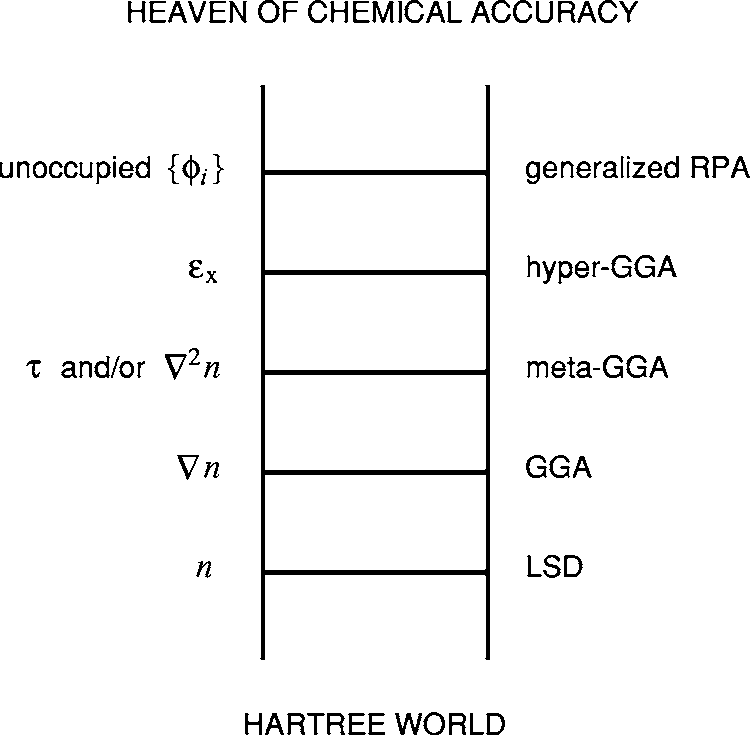
\includegraphics[width=0.9\textwidth]{gambar/jacob_ladder}
    \caption{Tangga Jacob dari pendekatan fungsional kerapatan terhadap energi korelasi-pertukaran. \citep{perdew2005}}
    \label{fig:xc_jacob_ladder}
\end{figure}

Fungsional pertukaran-korelasi \(E_{xc}[\rho]\) adalah komponen kunci dalam DFT karena mengkompensasi efek pertukaran dan korelasi yang tidak dapat diakomodasi secara eksplisit dalam persamaan Kohn-Sham.
Secara umum, fungsional ini dapat dituliskan sebagai:
\begin{equation}
    E_{xc}[\rho] = \int \rho(\mathbf{r})\,\varepsilon_{xc}\Big(\rho(\mathbf{r}), \nabla\rho(\mathbf{r}), \ldots\Big) \, d\mathbf{r},
\end{equation}
di mana \(\varepsilon_{xc}\) adalah energi pertukaran-korelasi per partikel yang biasanya diaproksimasi dengan metode Pendekatan Kerapatan Lokal (LDA) atau Pendekatan Gradien Umum (GGA) \citep{Perdew1996}.
Dalam pendekatan LDA, \(\varepsilon_{xc}\) diasumsikan hanya bergantung pada densitas lokal, sehingga sangat sesuai untuk sistem homogen atau dengan variasi densitas yang lambat.
Sedangkan GGA memperkenalkan koreksi gradien dari densitas untuk menangani sistem dengan perubahan densitas yang lebih tajam.
Selain itu, fungsional hibrida seperti B3LYP menggabungkan sebagian dari kontribusi eksak pertukaran dari metode Hartree-Fock dengan fungsional DFT, sehingga meningkatkan akurasi untuk berbagai sistem molekuler dan padat \citep{Becke1993}.
Penentuan fungsional \(E_{xc}[\rho]\) yang tepat merupakan tantangan utama dalam DFT, karena ketidaklengkapan dalam pemodelan pertukaran dan korelasi dapat mengakibatkan kesalahan sistematik dalam perhitungan sifat elektronik dan energi ikatan.
Oleh karena itu, penelitian berkelanjutan diarahkan pada pengembangan fungsional-fungsional baru yang dapat mengatasi keterbatasan LDA dan GGA, serta mengakomodasi efek korelasi yang lebih kompleks.

\subsection{Potensial Semu (Pseudopotentials)}
\begin{figure}[h!]
    \centering
    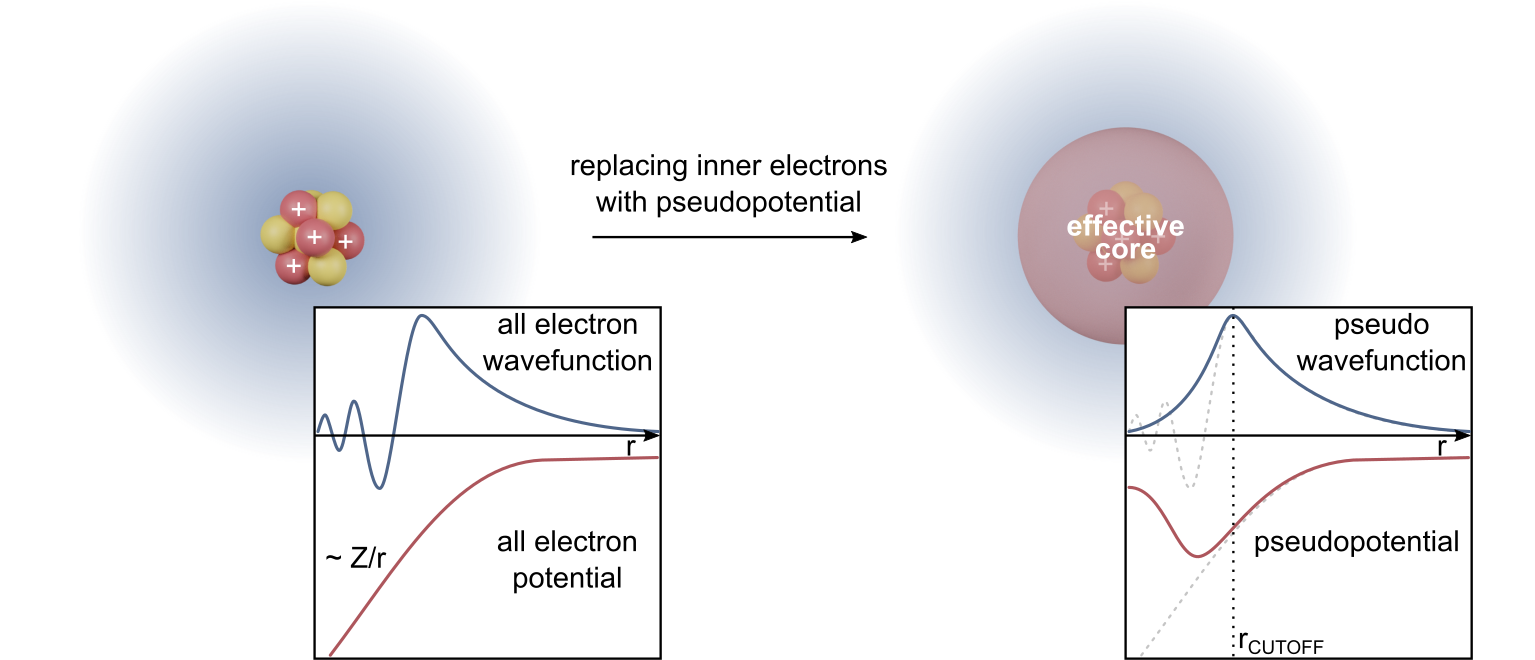
\includegraphics[width=0.9\textwidth]{gambar/pseudopotential}
    \caption{Visualisasi cara kerja pseudopotential \citep{pseudopotential}}
    \label{fig:pseudopotential}
\end{figure}
Dalam perhitungan DFT, salah satu tantangan utama adalah penanganan elektron inti yang memiliki variasi gelombang sangat cepat di sekitar nukleus.
Untuk mengatasi masalah ini, pendekatan potensial semu atau pseudopotentials diperkenalkan.
Ide dasarnya adalah menggantikan interaksi inti-elektron dengan suatu potensial efektif \(V_{ps}(\mathbf{r})\) yang secara signifikan menyederhanakan struktur gelombang elektron di daerah inti tanpa mengorbankan akurasi untuk elektron valensi:
\begin{equation}
    \left[-\frac{\hbar^2}{2m}\nabla^2 + V_{ps}(\mathbf{r})\right]\psi_i(\mathbf{r}) = \epsilon_i \psi_i(\mathbf{r}).
\end{equation}
Pseudopotentials memungkinkan penggunaan basis \emph{planewave} yang homogen dan efisien dalam ruang reciprocal, sehingga mengurangi beban komputasi.
Terdapat berbagai jenis pseudopotentials, seperti norm-conserving dan ultrasoft pseudopotentials, yang masing-masing memiliki keunggulan dan keterbatasan tersendiri.
Pemilihan jenis pseudopotential sangat bergantung pada sifat sistem yang dikaji serta tingkat akurasi yang diinginkan \citep{Payne1992}.
Selain mengurangi jumlah fungsi gelombang yang harus dihitung, pendekatan ini juga membantu menghindari ketidakstabilan numerik yang mungkin muncul akibat fluktuasi besar dalam fungsi gelombang di dekat inti.
Dengan demikian, pseudopotentials telah menjadi komponen penting dalam aplikasi DFT untuk material kompleks.

\subsection{Metode PAW (Projector Augmented-Wave)}
Metode PAW merupakan suatu pendekatan yang menggabungkan keunggulan metode pseudopotential dengan perhitungan \emph{all-electron} yang lebih akurat.
Metode PAW memperkenalkan fungsi proyekor dan fungsi tambahan (augmentation functions) untuk mengoreksi bentuk fungsi gelombang di daerah dekat inti, sehingga informasi mengenai nodal struktur asli dapat dipulihkan:
\begin{equation}
|\Psi_n\rangle = |\tilde{\Psi}_n\rangle + \sum_i \Big(|\phi_i\rangle - |\tilde{\phi}_i\rangle\Big) \langle \tilde{p}_i |
\tilde{\Psi}_n \rangle.
\end{equation}
Pendekatan ini memungkinkan perhitungan yang lebih akurat tanpa harus mengorbankan efisiensi komputasi secara signifikan.
Dengan PAW, perhitungan sifat-sifat elektron, terutama di daerah inti yang kritis bagi interaksi kimia, dapat dilakukan dengan lebih tepat.
Metode ini juga sangat berguna dalam menangani sistem dengan konfigurasi elektronik kompleks, misalnya pada material transisi atau sistem dengan cacat struktural \citep{Blochl1994}.
Secara konseptual, PAW dapat dilihat sebagai transformasi linear dari basis pseudopotential ke basis all-electron, yang menjaga keuntungan komputasi dari pendekatan pseudopotential sambil memulihkan informasi penting yang hilang pada daerah inti.

\subsection{Quantum Espresso}
Quantum Espresso merupakan salah satu paket perangkat lunak open-source yang populer untuk perhitungan DFT.
Perangkat lunak ini mengimplementasikan berbagai metode numerik, termasuk penggunaan basis \emph{planewave}, pseudopotentials, dan metode PAW, untuk menghitung struktur elektronik, energi total, serta sifat dinamik atomik dalam material \citep{Giannozzi2009}.
Paket Quantum Espresso dilengkapi dengan berbagai modul yang memungkinkan pengguna untuk melakukan perhitungan optimasi struktur, simulasi dinamika molekuler, serta analisis pita energi.
Selain itu, fleksibilitas dalam memilih fungsional pertukaran-korelasi, skema sampling ruang reciprocal, dan parameter kisi menjadikan perangkat lunak ini sangat berguna untuk penelitian material, terutama dalam studi material 2D dan sistem kompleks.
Dokumentasi dan komunitas pengguna yang luas juga mendukung pengembangan dan penerapan metode DFT yang lebih canggih.
Dalam praktiknya, input file Quantum Espresso memuat parameter-parameter penting seperti jenis fungsional XC, kriteria konvergensi, dan detail pseudopotentials yang digunakan, sehingga memungkinkan reproduksibilitas dan verifikasi hasil perhitungan di berbagai sistem studi.

%%%%%%%%%%%%%%%%%%%%%%%%%%%%%%%%%%%%%%%%%%%%%%%%%%%%%%%%%%%%%%
\section{Studi Lanjutan dan Pengembangan Metodologi}
Sebagai kelanjutan dari tinjauan pustaka di atas, sejumlah penelitian terbaru telah mengeksplorasi aspek tambahan pada material 2D serta mengembangkan metodologi komputasi yang semakin canggih.
Studi-studi ini tidak hanya memperkaya pemahaman kita terhadap sifat fundamental material 2D, tetapi juga memberikan kontribusi signifikan dalam peningkatan teknik simulasi dan perhitungan kuantum.
Penelitian mengenai sifat termal material 2D, misalnya, telah diteliti secara mendalam oleh \citep{Khan2017}, yang menunjukkan konduktivitas termal yang sangat tinggi pada grafena.
Temuan ini melengkapi studi sebelumnya dan membuka peluang untuk aplikasi pendinginan pasif dalam perangkat nanoelektronik.
Di samping itu, teori transport kuantum yang dikembangkan oleh \citep{Ando2002} menyediakan kerangka teoretis untuk memahami mobilitas dan perilaku elektron dalam sistem dua dimensi, yang sangat krusial untuk pengembangan perangkat berbasis 2D.
Analisis struktur dan cacat juga mengalami kemajuan melalui pendekatan eksperimental dan komputasional.
Penelitian oleh Zhang \citep{Zhang2020} dan \citep{Slotman2013} menyoroti peran penting cacat titik dalam memodifikasi sifat elektronik dan optik material 2D.
Selain itu, pendekatan representation-independent yang lebih baru, seperti yang diuraikan oleh \citep{Shen2022}, telah meningkatkan keakuratan perhitungan DFT untuk sistem dengan variasi densitas yang kompleks.
Dalam aspek kelistrikan, penelitian oleh Wang \citep{Wang2017} memberikan wawasan mengenai peningkatan performa elektronik melalui rekayasa heterostruktur, sedangkan studi oleh \citep{Munro2020} dan \citep{Huang2012} menyelidiki mekanisme pembentukan cacat dan pengaruhnya terhadap konduktivitas.
Pembaruan ulasan tentang material 2D juga disajikan oleh \citep{Bhimanapati2016}, yang memberikan gambaran menyeluruh mengenai tren riset di bidang ini.
Dari sisi manajemen termal, \citep{Khan2017} menekankan pentingnya pengendalian panas dalam perangkat nanoelektronik berbasis material 2D.
Sementara itu, metode komputasi juga terus berkembang dengan penerapan teknik \emph{machine learning} untuk prediksi sifat material, seperti yang ditunjukkan oleh \citep{Zheng2025}.
Studi mengenai cacat asli (\emph{native defects}) dalam material 2D juga mendapatkan perhatian melalui penelitian \citep{Weston2018}.
Dalam ranah simulasi komputer, karya klasik yang membahas algoritma dan metodologi MD tetap menjadi referensi penting.
Misalnya, karya \citep{Allen1989}, \citep{Rapaport2004}, dan \citep{Allen1989} terus dijadikan acuan dalam pengembangan metode simulasi dinamika molekuler.
Di sisi lain, peningkatan dalam perhitungan DFT melalui penggunaan fungsional hibrida telah didorong oleh penelitian \citep{Becke1993}, yang telah membuka jalan bagi pengembangan fungsional pertukaran-korelasi yang lebih akurat.
Sebagai tambahan, ulasan terbaru yang menyatukan berbagai pendekatan teoretis dan eksperimental juga memberikan kerangka kerja yang lebih holistik untuk mempelajari sifat-sifat sistem banyak partikel, seperti yang diuraikan dalam studi \citep{Lele2022}.
Dengan demikian, integrasi dari berbagai metodologi ini membentuk dasar yang kuat untuk penelitian material 2D di masa depan, serta memberikan landasan untuk pengembangan teknologi nanoelektronik yang lebih inovatif.
%%%%%%%%%%%%%%%%%%%%%%%%%%%%%%%%%%%%%%%%%%%%%%%%%%%%%%%%%%%%%%
% AKHIR DOKUMEN
%%%%%%%%%%%%%%%%%%%%%%%%%%%%%%%%%%%%%%%%%%%%%%%%%%%%%%%%%%%%%%%
